%
% File acl2013.tex
%
% Contact  navigli@di.uniroma1.it
%%
%% Based on the style files for ACL-2012, which were, in turn,
%% based on the style files for ACL-2011, which were, in turn, 
%% based on the style files for ACL-2010, which were, in turn, 
%% based on the style files for ACL-IJCNLP-2009, which were, in turn,
%% based on the style files for EACL-2009 and IJCNLP-2008...

%% Based on the style files for EACL 2006 by 
%%e.agirre@ehu.es or Sergi.Balari@uab.es
%% and that of ACL 08 by Joakim Nivre and Noah Smith

\documentclass[11pt]{article}
\usepackage{acl2013}
\usepackage{times}
\usepackage{url}
\usepackage{latexsym}
%\setlength\titlebox{6.5cm}    % You can expand the title box if you
% really have to

\title{Event extraction using iterative optimization}

\author{
   Aju Thalappillil Scaria \\
  {\tt ajuts@stanford.edu} \\\And
  Rishita Anubhai \\
  {\tt rishita@stanford.edu} \\\And
  Rose Marie Philip \\
  {\tt rosep@stanford.edu} 
\\}

\date{}

\begin{document}
\maketitle
\begin{abstract}
Abstract goes here
\end{abstract}

\section{Introduction}
\label{sec:introduction}
The World Wide Web is accessible to anyone with an internet connection. But analyzing this vast amount of data to extract meaningful information is rather difficult because of its sheer volume. There have been a lot of research focusing on extracting content from the web to build large knowledge bases. For instance, extracting events and the associated entities from biomedical and molecular biology text has drawn a lot of attention, especially because of the introduction of BIONLP tasks targeting fine-grained information extraction.  The knowledge bases built by information extraction systems can find application in a variety of fields, for example, to supplement the structured information available to build quiesting answering systems.

In this paper, we focus on the task of event and entity extraction, with semantic role labeling. Most of the prior work either focuses on subsets of these tasks or look at very specific types of events or entities that are to be extracted. For instance, Toutanova et. al. focuses on entity extraction and semantic role labeing assuming that the event triggeres are known, while McClosky focuses on event and argument extraction for only binding, regulation and phosphorylation event types. These works show that the task of extracting information from text is possible with reasonable accuracy level.  But, the performance of the state-of-the-art systems is still quite distant to that of a ’perfect’ extraction system. This is mostly because interpreting meaning from complex structures of natural language is a hard task. In this work, we combine the representations, feature extraction methods and models adopted in the previous work.

\section{Previous Work}
\label{sec:previousapproaches}
Most of the prevoius work dealt only with a subset of the three tasks listed as the project goals and dealt with very specific domains.  For instance, Chambers and Jurafsky ~\shortcite{chju2008} talks about event identification and temporal ordering using narrative event chains.Toutanova comes up with a joint model for argument extraction and semantic role labeling assuming that the trigger words are provided. Bjorne solves the problem of event extraction and semantic role labeling assuming the entities are known. Also, their event categories and arguments are closely tied to the BIONLP task and hence, would not generalize to domain-independent text. Chambers 2009 addresses the areas of event identification, and combines argument extraction with semantic role labeling using an unsupervised approach addressing narrative event chains in further detail. 

Different approaches have been tried to come up with a solution to these problems. While some work has used unsupervised learning methods (Chambers and Jurafsky 2008, 2009), there are others who viewed each task as a separate machine learning problem (Bjorne) or tried to combine the problems using joint models that can overcome the problem of cascading errors and does not have to assume independence of events and enitites (Toutanova and , Riedel and McCallum).

Events and entities have been represented in different ways; the work of Bjorne and McClosky and , Riedel and McCallum use graphs to represent relationship between events and entities, while Toutanova and McClosky, uses tree structure with classification of nodes as an entity or not. Also, some of the work rely on the constituency parse structure of sentences (Toutanova), while others ( Bjorne and McClosky) use the dependency parse structure for finding features. 




\section{Data and Evaluation}
\label{sec:data}
In this project, the dataset was prepared by annotating 125 paragraphs from different chapters of the text book {\em Biology (Eighth Edition)} by {\em Neil A. Campbell} and {\em Jane B. Reece}. Each paragraph is a text file and has an associated annotation file that indicates the different events and entities (by their character offsets in the original paragraph) and the event-entity and event-event relationships. The annotations were done by experts in the field (employees of the company Vulcan). Since there is not much data at our disposal, we split the data by a proportion of 70-30\% for training and testing. We randomly permute the order of files to avoid similarities in adjacent files and then use 10 fold cross validation on the training set. For event prediction, we use F1 score based on the trigger predictions made. In entity prediction, the F1 score is based on whether an entity was predicted correctly along with its association with the corresponding event.

\section{Model}
\label{sec:model}
In this section, we present the models we developed. We combine the learnings from the different approaches adoped in prior literature to build a model that can be used for event and entity extraction not specific to any domain. Even though our dataset is based on paragraphs from a biology textbook, we believe our models would generalize well to deal with more general content as our features and event/entity classes are not tied to the biological domain in any way. Our system takes a paragraph of text as input and does the following tasks:

\begin{enumerate}
\item Identify the events by locating the trigger words.
\item For each event, identify entities that are its arguments.
\item For each argument that is identified with a specific event, assign a semantic role.
\end{enumerate}

We model events and entities as sub-trees headed by a node in the constituency tree. Each sentence is assumed to be independent of each other as far as entity-event relationships are concerned. Events are denoted by their trigger words and are hence pre-terminals in the parse tree. Entities are denoted by a parse tree-node covering a sub-tree that spans over the whole text of the entity. In some cases when there is no single node that covers the entire entity (mostly because of parser errors, for e.g., PP attachment), we use an approximation by repeatedly removing tokens from the end or beginning of the span of text to identify a node that covers it. We manually verified that this heuristic works well in practice and results in entities that convey almost the full meaning of original span, and are well-formed.

In our project, we use Stanford Core NLP tools. We use the annotation pipeline available in the toolkit including tokenization, lemmatization, dependency and constituency parsers, and POS taggers. The events, entities and their relationships are represented as annotations on the already existing sentence annotations, by implementing the CoreAnnotation interface. This helps us to integrate our codebase with the existing features of the CoreNLP toolkit.

For all the classification tasks, we use maximum entropy model based on an implementation of L-BFGS for Quasi Newton unconstrained minimization. We use features based on the dependency graph of the sentence in conjunction with the constituency parse, since it contains information about the dependencies between tokens, which are critical in identifying event-entity relations. This is done by identifying the position of the headword of an entity or event from the dependency tree and analyzing the property of the head word. We use Collins head finding algorithm for finding the head word of a parse tree node. 

First, we present our model for task 1 which is an independent classification task. Then, we talk about task 2 where we identify entities that are arguments to event triggers. Since the information about entities can be used to improve event trigger prediction, we then cover the iterative optimization algorithm we developed that iteratively predicts event triggers from entities and entities from event triggers. Then, we talk about the joint re-ranking model we developed for semantic role labeling.
\label{sec:model}
\subsection{Event trigger prediction}
As we mentioned earlier, events are represented as pre-terminal nodes in the parse tree of a sentence. As a first step to the task, we built a baseline model that predicted every pre-terminal node whose part-of-speech tag started with 'VB' to be an event trigger. This model performed quite well giving an F1 score of 0.565, considering that it was a very naive approach. As the next step, we designed a MaxEnt model that trained on the annotated samples using several lexical and path features. The features we currently have include part-of-speech tag of the word, its lemma, the part-of-speech tag of its parent, the actual word itself and the path from root to the node. The results we have are in Table~\ref{table:eventprediction}. On doing error analysis, we found that our classifier fails to identify nominalized verb forms as event triggers. We used NomLex and NomBank, which are collections of nominalizations, to include a feature that indicates nominalization. NomLex proved useful and the classification accuracy improved quite significantly.

\label{sec:model}
\subsection{Argument identification for triggers}
An entity is represented as a node in the parse tree spanning over the full text of the entity along the leaves of the tree. The fact that there is more than one event in almost all sentences makes our task of event-entity association harder. This is because, instead of just predicting a node in the parse tree as an entity, we have to predict if a node is associated with a specific trigger from task 1. To overcome this, we assign a probability for each node in the parse tree to be an entity associated with each event. If $N$ is the set of $n$ nodes $\{t_1, t_2, ... t_n\}$ in the parse tree, given an event trigger $e$, our goal is to predict the best set of entities $A$ for $e$.

As a first step, we built a baseline model that predicts a node in the parse tree as an argument to an event trigger, if it is of part-of-speech tag 'NP' and if the head word of the node in the parse tree is a child of the event trigger in the dependency tree of the sentence. We used Collins head finder algorithm to identify the headword of a parse tree node. We then implemented a MaxEnt based model using more features between the event triggers and the candidate nodes to classify the node as either an argument or $NONE$ if not. This is also a local model, hence

$P_{A}(A | e, x) = \prod_{t_{i}\in N} P_{A}(t_{i} | e, x) $

The features we use for finding event arguments are combinations of features of both event node and the candidate entity node. This includes POS tag of candidate + POS tag of event trigger, headword of candidate + POS tag of event trigger, path from the candidate to the event trigger and an indicator feature denoting whether the headword of the candidate is a child of the trigger in the dependency tree. The model assigns a probability value for each node in the parse tree to be an argument to a specific event trigger.

{\bf Dynamic Program for non-overlapping constraint.} Since we predict a node in the parse tree as an argument to an event trigger or not, there are instances when predicted entities overlap. For instance, a sub-tree of a tree node already marked as an entity may also be tagged as an entity. To avoid this, we devised a bottom-up dynamic program that tags a node as entity or not, looking at the probability of the node and its immediate children being entities. The dynamic program works from the pre-terminal nodes of the tree and find best assignments for each tree using the already computed assignments for its children. This ensures that a sub-tree that is a part of $A$ in itself doesn't have smaller subtrees that belongs to $A$. The most likely assignment for a tree $t$  to $A$ or $NONE$ is the one that corresponds to the maximum of:

\begin{enumerate} 
\item The sum of the log-probabilities of the most likely assignments of the children sub-trees $t_1, t_2,.. t_k$, plus the log-probability for assigning the node $t$ to $NONE$.
\item The sum of the log-probabilities for assigning all of $t_i$'s nodes to $NONE$ plus the log-probability of assigning the node $t$ to $A$.
\end{enumerate}

Another addition we did to the dynamic program was that an entity node cannot subsume a node in the parse tree that is an event trigger.
\label{sec:model}
\subsection{Iterative Optimization Algorithm}
One of the drawbacks of our approach to event trigger and argument prediction was that the models were independent. As a result, any errors made in trigger prediction will cascade and affect the argument identification phase. For instance, if an event trigger is not predicted, we are going to miss all the argument predictions for the trigger as well. At the same time, any incorrect event triggers predicted may result in lots of event-argument pairs being predicted that do not exist. Even after we used NomLex to find nominalizations, our classifier missed predicting some of the triggers. But, if we knew that there were entities that were children of the word in the dependency graph, then it gives more evidence that the word is an event trigger. At the same time if there are words that we might have predicted as triggers that do not have any entities as children in the dependency tree, they are less likely to be even triggers. Hence, we hypothesized that knowledge about entities in the sentence can help in event trigger prediction as we can use more features from the dependency tree. To test this, we used the gold entities from a sentence to add more features for event trigger prediction and we found that it gave us a boost in F1 score from 0.68 to 0.82. Since gold entities are not available during the test phase, we designed a separate model that predicts entities in a sentence independent of the triggers. As before, entities are sub-trees under a parse tree node and the model predicts the probability of a node to be an entity or not. We used the head word of the span covered by the node, its POS tag, its parents POS tag, the path to the node in the parse tree and the CFG rule expansion of its parent as features. We used the same dynamic programming approach for non-overlapping constraints of entities.

\begin{figure}[t]
	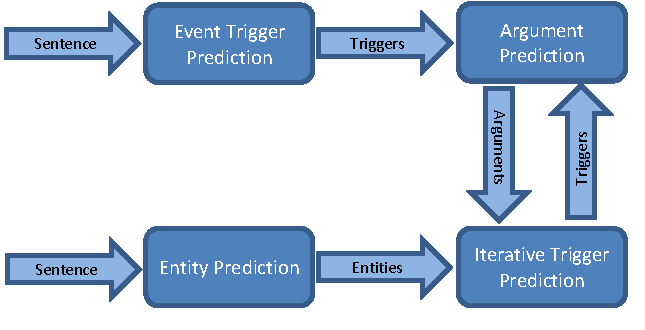
\includegraphics[width=1\columnwidth]{Images/IO}
	\caption{Stages in iterative optimization algorithm}
	\label{fig:iosteps}
\end{figure}

The different stages involved in the iterative optimization algorithm is depicted in Figure~\ref{fig:iosteps}. We use the event triggers predicted to predict its arguments. Now, we combine the set of entities predicted as arguments, with those predicted by the independent argument prediction model to create the set of all entities and is used in trigger prediction. This model predicts the most likely labeling $T$ that maximizes

$P(T | x, A) = \prod_{e_{i}\in N_{pt}} P(e_{i}\in TRIG | x, A) $, where $TRIG$ and $A$ are as defined earlier.

Once this models predicts the event triggers, we use the same model $P(A | e,x)$ to predict arguments associtated with each event trigger that satisfy the non-overlapping constraint. We repeat the iterative trigger and argument prediction till there is no improvement in F1 score.

The mode $P(T | x, A)$ uses the path to entities in parse tree, path length to the nearest entity, the acutal path to nearest entity and the number of words between closest entity before and after the node as features.

\label{sec:model}
\subsection{Semantic Role Labeling}
For argument identification, we had used a binary classifier based on MaxEnt model that predicts a probability value for it to be an argument. For semantic role labeling, we extended this model to a multi-class classifier to generate probability values for a parse-tree node being assigned to a specific semantic role. We also modified the dynamic program for non-overlapping constraint used in argument prediction to a re-ranking model that jointly assigns semantic role to all nodes in a sub-tree. Let $L$ be a labeling of semantic roles to the parse tree nodes, including $NONE$ if it is not an entity. Our goal is to maximize the probability of the labeling we generate.

We use a bottom up re-ranking approach by keeping the top-k joint assignment of semantic roles to all nodes in a sub-tree. This algorithm is similar to the dynamic programming for non-overlapping constraints. At the pre-terminal nodes, we keep just the semantic roles of the word subsumsed by the node in descending order of probability. At nodes above the pre-terminal nodes, there are two scenarios:

\begin{enumerate}
\item The node is an argument to the trigger: In this case, the node has a non-NONE semantic role and none of the children nodes can be entities and hence all children would have semantic role $NONE$. For each non-NONE semantic role of the node, we compute the probability value of the joint labeling of the sub-tree.
\item The node is not an argument to the trigger: In this case, the node has a semantic role of $NONE$. Since at each of the child nodes we have top-k possible assignments, we take all combinations of assignments of children nodes and compute the probability for each of these possible joint labeling.
\end{enumerate}

The next step is to re-rank these possible joint assignments at the node and then retain only the top-k at the node. This algorithm proceeds until we reach the root and the joint labeling that has the highest probability will be the semantic roles predicted by the model. We are currently using k=5 in our model.

\section{Results}
\label{sec:results}

\begin{table}
\centering
\begin{tabular}{|l||c|c|c|} \hline
&\textbf{Precision} & \textbf{Recall} & \textbf{F1} \\ \hline
\hline
Baseline& 0.421 & 0.703 &0.525\\
MaxEnt\_Basic& 0.766 & 0.644&  0.691 \\
MaxEnt\_IO&0.747&0.668&0.699\\
\hline
\end{tabular}
\caption{Event trigger prediction}
\label{table:eventprediction}
\end{table}

\begin{table}
\centering
\begin{tabular}{|l||c|c|c|} \hline
&\textbf{Precision} & \textbf{Recall} & \textbf{F1} \\ \hline
\hline
MaxEnt\_Oracle&0.719&0.561&0.629\\
Baseline&0.482&0.536&0.504\\
MaxEnt\_Basic&0.606&0.437&0.505\\
MaxEnt\_IO&0.577&0.477&0.519\\
\hline
\end{tabular}
\caption{Entity prediction for event triggers (Oracle)}
\label{table:entityprediction}
\end{table}

\begin{table}
\centering
\begin{tabular}{|l||c|c|c|} \hline
&\textbf{Precision} & \textbf{Recall} & \textbf{F1} \\ \hline
\hline
Baseline&0.&0.&0.\\
MaxEnt\_Oracle&0.&0.&0.\\
MaxEnt\_Basic&0.&0.&0.\\
MaxEnt\_IO&0.&0.&0.\\
\hline
\end{tabular}
\caption{Semantic role labeling}
\label{table:srlprediction}
\end{table}

The results for event prediction tasks are presented in Table~\ref{table:eventprediction}. The baseline model that predicted every verb as an event trigger performed quite well giving an F1 score of 0.565.

TODO - Talk about the results for event and entity prediction.

The results for argument prediction are presented in Table~\ref{table:entityprediction}. The baseline model intuitively captures the relation between event triggers and its arguments as is evident from the F1 score of 0.593 achieved using a relatively simple approach. Results after using DP - The dynamic programming approach gave us a boost of 0.04 (0.60 to 0.64) in F1 score. 

The results for semantic role labeling are presented in Table~\ref{table:srlprediction}. The baseline model predicts the most frequent semantic role as the role of an entity.

\section{Analysis}
\label{sec:analysis}
In section, we analyze the results in detail and perform error analysis. First we talk about the general points and later we talk about each tasks in detail

{\bf Lexical vs Non-lexical featuers -} Using lexical features helps to capture words or phrases that are repeating. At the same time, using features based on the POS tags and path in the parse tree or dependency tree helps us to identify structural traits. Since our training data was limited, using lexical features alone wasn't really helpful because most of the words and phrases were non-repeating. At the same time, adding many features based on path resulted in high precision but low recall. So, we've adopted a mix of both lexical and non-lexical features.

{\bf Annotation errors -} There were many instances when we thought the annotations were not correct. For example, events like 'transposition' and 'duplication' were not marked as a triggers in some sentences, maybe, because those were not important events according to the annotator. Also, while marking phrases that constitute an entity, there were many instances when multiple annotations were possible. This raises an import concern with all manually annotated corpora - that choices of annotations are subjective.

{\bf Parser errors-} Since many of the features that we used are based on the parses generated for a sentence, any mistakes by the parser would automatically result in misclassifications of event and entities. A typical example is problems arising due to PP attachment of phrases that were marked as entities.

\subsection{Event trigger prediction}
{\bf Verb Nominalizations -} Most of the event triggers are verbs which makes it easy to achieve F1 scores of around 0.6 without many features. But, including features to classify nominalized verbs that are event triggers is a hard task. Especially because there is no single source of word nominalizations that is perfect. We tried NomLex and NomBank, which are collections of nominalizations. NomLex proved useful and the classification accuracy improved by around 2-3\%. But, since NomLex was not an extensive dictionary, some nominalizations were still misclassified. Using WordNet derivations helped us to counter this and to improve the performance by another 2\%. After including the features for word nominalizations, the model now identifies event triggers like 'effect', 'change', 'impact', 'degradation', 'concentration' etc. as event triggers. At the same time, there are many instances when nouns get tagged as event triggers even when they were not event triggers, for instance 'damage' was tagged as trigger from the phrase 'strand containing the damage'. Also, more complex nominalizations like 'synthesis', 'bronchitis' etc. were missed.

{\bf Iterative Optimization -} The iterative optimization algorithm we developed was quite efficient in correcting some of the mistakes made by the basic trigger prediction algorithm. As an example, in the sentence, {\em The original cell produces a copy of its chromosome and surrounds it with a tough multilayered structure, forming the endospore.}, 'copy' was predicted as an event trigger, possibly because of strong lexical features. But, this gets corrected with the iterative algorithm as it does not have any child entities in the dependency tree. Similarly, in the sentence, {\em Each gene on one homolog is aligned precisely with the corresponding gene on the other homolog.}, 'aligned' was not initially predicted as an event trigger, but the iterative algorithm predicts it as a trigger.

We feel that including word clustering features that cluster together words that are semantically close would help us solve the problems arising with sparsity of labeled data.

\subsection{Entity prediction}
The task of argument prediction is a much harder task as evident from the lower F1 scores, mainly because of two reasons. Firstly, entities that are arguments to event triggers are phrases and marking boundaries of entities are subjective. We partly overcame this difficulty by modeling entities as parse tree nodes and devising a dynamic program for enforcing non overlapping constraints. The dynamic programming approach gave us a boost of around 4\% in F1 score. Secondly, since we are now scoring event-entity combinations, identifying correct triggers to connect the entity to is a hard problem, especially in the cases when an entity is shared between two triggers or when the entities and trigger words are far apart in the sentence. We tried to overcome this by introducing features based on dependency parse structure of sentences as well.

TODO - Why does IO reduce precision?

\subsection{Semantic role labeling}

TODO - Finish this section

\section{Conclusion}
\label{sec:conclusion}
Event extraction is a promising area of research that will find a lot of application with the ever-increasing amount of data being generated with the increase in both newly published material and also with many popular books and articles being converted to electronic format. In this paper, we present a set of models for event and entity extraction with semantic role labeling. We have a basic trigger prediction model and an entity prediction model that predicts event triggers. Since we found that knowledge of entities can help to predict event triggers, we devised the iterative optimization algorithm that iteratively improves trigger and its argument prediction. Following this, we developed a dynamic programming approach for semantic role labeling.

We feel that combining the features from parse tree and dependency tree is something that hasn't been extensively used before and it proves very helpful. Also, the iterative approach to event and entity prediction works well considering the simplicity of the model. Further work would include adding semantic role labeling also into the iterative algorithm and also to include a temporal ordering of events to form a chain of events making a story.

\section*{Acknowledgments}

Do not number the acknowledgment section. Do not include this section when submitting your paper for review.

%\bibliographystyle{acl}
%\bibliography{bibliography}
\begin{thebibliography}{}

\bibitem[\protect\citename{Chambers and Jurafsky}2008]{chju2008}
Nathanael Chambers and Dan Jurafsky.
\newblock 2008.
\newblock Unsupervised learning of narrative event chains.
\newblock In {\em Proceedings of ACL-08}.

\bibitem[\protect\citename{Chambers and Jurafsky}2009]{chju2009}
Nathanael Chambers and Dan Jurafsky.
\newblock 2009.
\newblock Unsupervised Learning of Narrative Schemas and their Participants
\newblock In {\em Proceedings of ACL-09}.

\bibitem[\protect\citename{Chambers and Jurafsky}2011]{chju2011}
Nathanael Chambers and Dan Jurafsky
\newblock 2011.
\newblock Template-Based Information Extraction without the Templates
\newblock In {\em Proceedings of ACL-11}.

\bibitem[\protect\citename{Bjorne \bgroup et al.\egroup}2009]{bjorne}
Jari Bjorne, Juho Heimonen, Filip Ginter, Antti Airola, Tapio Pahikkala, Tapio Salakoski
\newblock 2009.
\newblock Extracting Complex Biological Events with Rich Graph-Based Feature Sets.
\newblock In {\em Proceedings of the Workshop on BioNLP: Shared Task,}.

\bibitem[\protect\citename{Toutanova \bgroup et al.\egroup}2005]{toutanova}
Kristina Toutanova, Aria Haghighi, Christopher D. Manning
\newblock 2005.
\newblock Joint Learning Improves Semantic Role Labeling.
\newblock In {\em Proceedings of ACL 2005}.

\bibitem[\protect\citename{Riedel and McCallum}2008]{riedelmc}
Sebastian Riedel Andrew McCallum
\newblock 2008.
\newblock Fast and Robust Joint Models for Biomedical Event Extraction.
\newblock In {\em Proceedings of the 2011 Conference on Empirical Methods in Natural Language Processing}.

\bibitem[\protect\citename{Miwa \bgroup et al.\egroup}2010]{miwa2010c}
Makoto Miwa, Rune Saetre, Jin-Dong D. Kim, and Jun’ichi Tsujii
\newblock 2010c.
\newblock Event extraction with complex event classification using rich features
\newblock In {\em Journal of bioinformatics and computational biology}.

\bibitem[\protect\citename{McClosky \bgroup et al.\egroup}2011]{mcclosky}
David McClosky, Mihai Surdeanu, and Christopher D. Manning
\newblock 2011.
\newblock Event Extraction as Dependency Parsing
\newblock In {\em Proceedings of ACL-11}.

\bibitem[\protect\citename{Chambers and Jurafsky}{2008-temporal ordering}]{temporalordering}
Nathanael Chambers and Dan Jurafsky
\newblock 2008.
\newblock Jointly Combining Implicit Constraints Improves Temporal Ordering
\newblock In {\em EMNLP-08}.

\bibitem[\protect\citename{McCloskly \bgroup et al.\egroup}2012]{quang}
Quang Xuan Do, Wei Lu, Dan Roth
\newblock 2012.
\newblock Joint Inference for Event Timeline Construction
\newblock In {\em EMNLP-12}.

\end{thebibliography}
\end{document}
